\section* {1.1  LU -  разложение матриц}

\subsection{Постановка задачи}
Реализовать алгоритм LU -  разложения матриц (с выбором главного элемента) в виде программы. Используя разработанное программное обеспечение, решить систему линейных алгебраических уравнений (СЛАУ). Для матрицы СЛАУ вычислить определитель и обратную матрицу. 

{\bfseries Вариант:} 24

\begin{cases}
& -7x_1-2x_2-x_3-4x_4 = -12 \\
& -4x_1+6x_2 - 4x_4 = 22 \\
& 8x_1+2x_2-9x_3-3x_4 = -51 \\
& -7x_1+x_4 = 49 \\
\end{cases}
%\pagebreak

\subsection{Результаты работы}
\begin{figure}[h!]
\centering
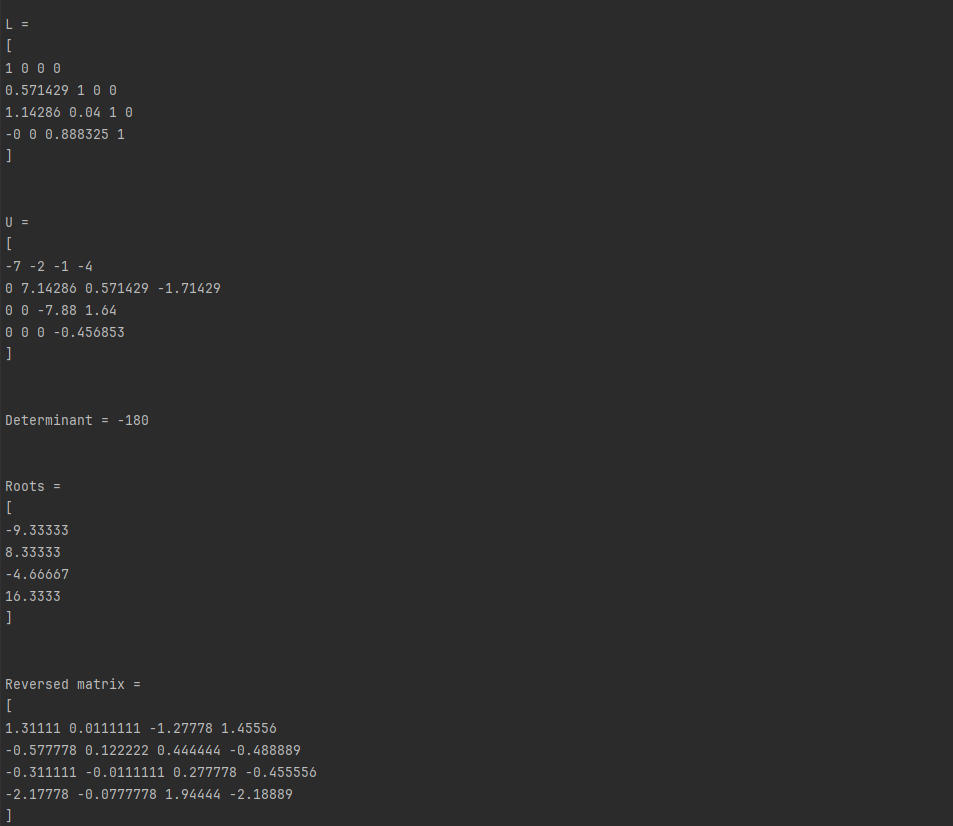
\includegraphics[width=15cm, height=10cm]{img/lab1_1_res.png}
\caption{Вывод программы в консоли}
\end{figure}
\pagebreak

\subsection{Исходный код}

\lstinputlisting{include/lab1_1/main.cpp}
\lstinputlisting{include/lab1_1/matrix.cpp}
\lstinputlisting{include/lab1_1/matrix.hpp}


\section* {1.2  Метод прогонки}

\subsection{Постановка задачи}
Реализовать метод прогонки в виде программы, задавая в качестве входных данных ненулевые элементы матрицы системы и вектор правых частей. Используя разработанное программное обеспечение, решить СЛАУ с трехдиагональной матрицей.  

{\bfseries Вариант:} 24

\begin{cases}
& -11x_1+9x_2 = -117 \\
& -9x_1+17x_2+6x_3 = -97 \\
& 5x_2+20x_3+8x_4= -6 \\
& -6x_3-20x_4+7x_5 = 59 \\
& 2x_4+8x_5 =-86\\
\end{cases}
% \pagebreak

\subsection{Результаты работы}
\begin{figure}[h!]
\centering
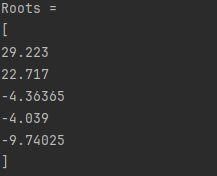
\includegraphics[width=.7\textwidth]{img/lab1_2_res.png}
\caption{Вывод программы в консоли}
\end{figure}
\pagebreak

\subsection{Исходный код}
\lstinputlisting{include/lab1_2/main.cpp}
\lstinputlisting{include/lab1_2/matrix.cpp}
\lstinputlisting{include/lab1_2/matrix.h}


\pagebreak
\section* {1.3  Метод простых итераций. Метод Зейделя}

\subsection{Постановка задачи}
Реализовать метод простых итераций и метод Зейделя в виде программ, задавая в качестве входных данных матрицу системы, вектор правых частей и точность вычислений. Используя разработанное программное обеспечение, решить СЛАУ. Проанализировать количество итераций, необходимое для достижения заданной точности. 

{\bfseries Вариант:} 24

\begin{cases}

& -25x_1+4x_2-4x_3+9x_4 = 86 \\
& -9x_1+21x_2+5x_3-6x_4 = 29 \\
& 9x_1+2x_2+19x_3-7x_4 = 28 \\
& -7x_1+4x_2-7x_3+25x_4 = 68 \\
\end{cases}
% \pagebreak

\subsection{Результаты работы}
\begin{figure}[h!]
\centering
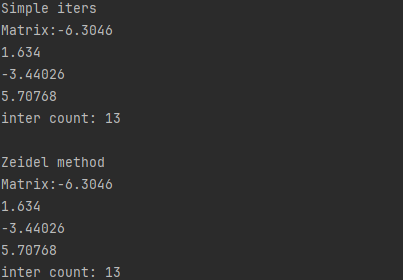
\includegraphics[width=15cm, height=10cm]{img/lab1_3_res.png}
\caption{Вывод программы в консоли}
\end{figure}

% \vfill

\pagebreak

\subsection{Исходный код}
\lstinputlisting{include/lab1_3/main.cpp}
\lstinputlisting{include/lab1_3/matrix.cpp}
\lstinputlisting{include/lab1_3/matrix.h}


\pagebreak
\section* {1.4  Метод вращений}

\subsection{Постановка задачи}
Реализовать метод вращений в виде программы, задавая в качестве входных данных матрицу и точность вычислений. Используя разработанное программное обеспечение, найти собственные значения и собственные векторы симметрических матриц. Проанализировать зависимость погрешности вычислений от числа итераций. 

{\bfseries Вариант:} 24

  \begin{pmatrix}
    -8 & -4 & 8 \\
    -4 & -3 & 9 \\
    8 & 9 & -5
  \end{pmatrix}
% \pagebreak

\subsection{Результаты работы}
\begin{figure}[h!]
\centering
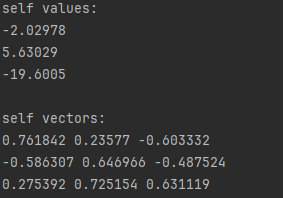
\includegraphics[width=.9\textwidth]{img/lab1_4_res.png}
\caption{Вывод программы в консоли}
\end{figure}

\pagebreak

\subsection{Исходный код}
\subsection{/main.cpp}
\lstinputlisting{include/lab1_4/main.cpp}
\lstinputlisting{include/lab1_4/matrix.cpp}
\lstinputlisting{include/lab1_4/matrix.h}





\pagebreak
\section* {1.5  QR – разложение матриц}

\subsection{Постановка задачи}
Реализовать алгоритм QR – разложения матриц в виде программы. На его основе разработать программу, реализующую QR – алгоритм решения полной проблемы собственных значений произвольных матриц, задавая в качестве входных данных матрицу и точность вычислений. С использованием разработанного программного обеспечения найти собственные значения матрицы.


{\bfseries Вариант:} 24

  \begin{pmatrix}
    -3 & 1 & -1 \\
    -6 & 9 & -4 \\
    5 & -4 & -8
  \end{pmatrix}
% \pagebreak

\subsection{Результаты работы}
\begin{figure}[h!]
\centering
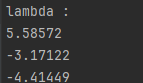
\includegraphics[width=.9\textwidth]{img/lab1_5_res.png}
\caption{Вывод программы в консоли}
\end{figure}

\pagebreak

\subsection{Исходный код}
\lstinputlisting{include/lab1_5/main.cpp}
\lstinputlisting{include/lab1_5/matrix.cpp}
\lstinputlisting{include/lab1_5/matrix.h}

